\documentclass[conference]{IEEEtran}
\usepackage{cite}
\usepackage{graphicx}
\usepackage{amsmath,amssymb,amsfonts}
\usepackage{textcomp}
\usepackage{url}
\usepackage[hidelinks]{hyperref}
\usepackage{xcolor}
\emergencystretch=3em
\setcounter{dbltopnumber}{2}
\renewcommand{\dbltopfraction}{0.95}
\renewcommand{\dblfloatpagefraction}{0.85}
\renewcommand{\textfraction}{0.05}
\newcommand{\CADDAM}{CADD\allowbreak{}+\allowbreak{}AlphaMissense}
\newcommand{\GCNCADDAM}{GCN\allowbreak{}+\allowbreak{}CADD\allowbreak{}+\allowbreak{}AlphaMissense}

\title{Auditing Fixed Protein-Feature Propagation on STRING Networks for Missense Variant Pathogenicity Prediction}

\author{}

\begin{document}
\maketitle


\begin{abstract}
\bfseries\boldmath
Network propagation can improve protein representations without establishing that network topology provides independent variant-level information. We audit fixed two-hop protein-feature propagation (FPP), with no learned graph parameters, on a shared STRING functional-association network. The reconstructed dataset contains 177,213 ClinVar missense variants mapped to 14,123 labelled proteins in a 19,622-node graph. Across three classifier seeds, FPP increased mean AUC from 0.7835 to 0.7950 and mean AUPRC from 0.6116 to 0.6484 over raw ESM representations. Protein-clustered bootstrap of a retained reference run widened both gain intervals across zero. Direct-edge ablation and topology permutation produced lower scores, although their training seeds and epoch budgets differ from the full-graph comparison. Architecture-matched fusion with CADD and AlphaMissense retained substantial gains using raw ESM and graph controls; the smaller real-network margins over edge-ablated and permuted fusion had intervals crossing zero. These intervals do not establish equivalence. The homology-aware graph-fusion result is a single-run descriptive stress test. Post-hoc complete-case evaluation preserved the original-split fusion ordering, whereas error-transition balances changed across decision thresholds. Topology-selected subgroups remain exploratory. The audit identifies evaluation sensitivities of this fixed, transductive representation pipeline; it does not establish a limit on learned graph models or prospective clinical performance.

\end{abstract}

\begin{IEEEkeywords}
\bfseries\boldmath
Missense variant pathogenicity, STRING networks, fixed feature propagation, protein language models, evaluation audit.
\end{IEEEkeywords}

\section{Introduction}

Missense variant pathogenicity prediction has been advanced by established methods such as CADD, REVEL, MVP, PrimateAI, EVE and AlphaMissense \cite{Kircher2014CADD,Ioannidis2016REVEL,Qi2021MVP,Sundaram2018PrimateAI,Frazer2021EVE,Cheng2023AlphaMissense}, as well as by protein language models such as ESM \cite{Lin2023ESM}. These approaches capture sequence, evolutionary and annotation-derived signals. Disease-associated proteins are also embedded in molecular interaction networks, and disease-associated mutations can perturb protein-protein and other macromolecular interactions \cite{Barabasi2011NetworkMedicine,Menche2015DiseaseModules,Sahni2015InteractionPerturbation,Chen2018InteractomePerturbation}. PPI graphs provide an additional source of context for missense variant prediction.

Earlier approaches incorporated protein-interaction and other molecular-network features into single-amino-acid variant prioritization, showing that network context can provide information complementary to sequence, structure and annotation features \cite{Yates2014SuSPect,Ozturk2022NetworkFeatures}. More recent graph-based variant predictors include graph attention models for missense effects, heterogeneous gene-variant graph approaches, multimodal variant graph methods and disease-specific graph models \cite{Zhang2022gMVP,Cheng2021VEGN,Yu2025GNNMAP,Ghadie2025DiseaseSpecificGNN}. These studies establish the relevance of relational structure to variant interpretation. We focus on how to interpret gains obtained by propagating protein language model embeddings over a shared STRING association graph before variant-level classification.

A shared-graph setting mixes several effects. Train, validation and test variants may have distinct protein identifiers while their proteins remain directly connected in the same STRING graph. Related proteins may also cross partitions when homology is not explicitly controlled \cite{Littmann2022ProteinMLTips,Teufel2023GraphPart}. Strong variant-effect predictors such as CADD and AlphaMissense can further reduce the marginal contribution of graph propagation. We evaluate protein-topology correspondence, graph connectivity, protein-level uncertainty, homology-aware performance and complementarity to established predictors.

We audit raw ESM, fixed propagation, external scores and fusion models on a reconstructed ClinVar-STRING dataset. The contribution is an evaluation study: it combines graph-intervention controls with capacity-matched fusion and protein-clustered uncertainty, documents sensitivities to split and comparison protocol, and describes exploratory topology and error-transition profiles. The audit does not introduce a new predictor or cover trained message-passing architectures.

\section{Materials and Methods}

\subsection{Dataset and graph construction}

ClinVar variant annotations were obtained from the official NCBI ClinVar FTP tab-delimited variant-summary file \cite{Landrum2020ClinVar}. We used the ClinVar variant-summary release dated 31 March 2024 and retained checksums for the exact input file used in the reconstruction. We reconstructed a filtered, non-conflicting missense dataset and mapped variants to STRING human protein identifiers. We retained GRCh38 germline missense SNVs with criteria-supported review status, combined pathogenic and likely pathogenic records into the positive class, combined benign and likely benign records into the negative class, removed uncertain or conflicting records, and collapsed duplicate VariationIDs. The final ClinVar-STRING dataset contained 177,213 missense variants mapped to 14,123 labelled STRING proteins. The propagation graph contained 19,622 STRING protein nodes and 13,715,404 directed edge-index entries from the STRING v12 protein-association network \cite{Szklarczyk2023STRING}. We used this network as STRING network context; its association evidence extends beyond direct physical interactions.

\subsection{Protein representations and fixed propagation}

Raw protein features were generated using the ESM-2 650M checkpoint, with 1,280-dimensional protein-level vectors obtained by residue averaging \cite{Lin2023ESM}. Fixed protein-feature propagation (FPP) was computed by two-hop GCN-style propagation over the normalized STRING graph \cite{Kipf2017GCN}. FPP has no learned graph-convolution parameters; the downstream MLP alone was trained. Fixed propagation isolates topology-induced smoothing from capacity gains due to trainable graph layers and provides a controlled representation for the audit. Let $X$ denote the raw ESM protein-representation matrix. The implementation symmetrized the retained edge list, added self-loops and coalesced duplicate edges. After self-loop addition, let $\tilde{A}$ denote the binary adjacency matrix and $\tilde{D}$ its degree matrix. We computed the symmetrically normalized adjacency matrix as
\begin{equation}
\hat{A}=\tilde{D}^{-\frac{1}{2}}\tilde{A}\tilde{D}^{-\frac{1}{2}},
\end{equation}
\begin{equation}
H=\frac{1}{3}\left(X+\hat{A}X+\hat{A}^{2}X\right).
\end{equation}
The fixed two-hop FPP representation $H$ averages the original ESM features, one-hop and two-hop STRING-smoothed features. Propagation used only graph structure and ESM features; downstream classification used the representation of each variant's mapped STRING protein. The full graph contained train, validation and test nodes with their ESM features, making the evaluation transductive. Held-out features and graph structure were available during propagation, but held-out labels were not used. Embedding-only models assign identical inputs to variants mapped to the same protein; they cannot resolve residue-specific effects within that protein.

\subsection{Splits, classifiers and external predictors}

The original split assigned train, validation and test variants by STRING protein ID, with no shared proteins across partitions. The split contained 141,864 training variants, 17,129 validation variants and 18,220 test variants. The homology-aware split used MMseqs-derived protein clusters, assigned each cluster wholly to one partition by greedy balancing of variant-row counts, without label-prevalence stratification, and preserved the same row counts \cite{Steinegger2017MMseqs2}. We use this split as a stress test. Its test positive rate was 10.56\%, compared with 31.95\% in the original split, which limits direct cross-split AUPRC comparison.

All representation and fusion models were evaluated with a downstream MLP classifier selected by validation AUC and optimized with Adam \cite{Kingma2015Adam}. Multi-feature representation and fusion models used a 512/128 hidden-layer MLP with dropout 0.3. Low-dimensional external-score baselines used a smaller 32/16 classifier with dropout 0.2. Architecture-matched \CADDAM{} and fusion-control comparisons used the 512/128 classifier to keep downstream capacity matched. Training used mini-batches of 1,024 variants, learning rate $10^{-3}$, weight decay $10^{-5}$, a nominal maximum of 50 epochs (30 for the representation edge-ablation and topology-permutation controls; Supplementary Table 8) and early stopping after five consecutive validation checks without improvement in validation AUC. Class imbalance was handled with \texttt{BCEWithLogitsLoss} using training-partition positive-class weight $N_{\mathrm{negative}}/N_{\mathrm{positive}}$. CADD GRCh38 v1.7 scores and AlphaMissense hg38 scores were matched to the reconstructed variants \cite{Kircher2014CADD,Schubach2024CADDv17,Cheng2023AlphaMissense}. CADD scores covered 177,205 variants (99.995\%), and AlphaMissense scores covered 171,753 variants (96.92\%). Missing CADD and AlphaMissense scores were imputed with training-set medians; AlphaMissense-based feature sets also included a binary missingness indicator. In the evaluated MLP configurations, no additional z-score standardization was applied to CADD, AlphaMissense or embedding-derived inputs. All architecture-matched fusion controls shared the same preprocessing and feature construction. Alternative feature-scaling strategies were not evaluated. The main repeated comparisons used seeds 42, 43 and 44; representation-level negative controls used different seeds and are not matched repeats (Supplementary Table 8).

\subsection{Audit analyses}

Uncertainty was assessed using variant-level bootstrap and protein-clustered bootstrap \cite{Efron1993Bootstrap}. Connectivity tests removed direct train-test STRING edges and regenerated FPP embeddings. Partial edge-ablation curves removed 0\%, 25\%, 50\%, 75\% and 100\% of direct train-test protein pairs using random removal, higher-STRING-score-first removal and lower-STRING-score-first removal. Topology permutation preserved the unlabeled graph structure and randomized the correspondence between protein identity and graph position, testing whether generic graph smoothing explained the gain. Fusion controls concatenated \CADDAM{} features with raw ESM, edge-ablated FPP and topology-permuted FPP representations, testing representation complementarity and sensitivity to protein-topology correspondence. Edge removal also changes normalization and retains indirect cross-partition paths; it does not isolate a causal contribution of direct connectivity.

Topology-context analyses stratified test variants by degree, k-core, betweenness, clustering coefficient, neighbour-risk and community-boundary features. Neighbour-risk and neighbour pathogenic-rate features for validation and test proteins were computed from training-set labels only; validation and test labels were not used to construct these topology-context features. Corrected-sample analyses compared variants whose predictions were corrected or degraded after adding graph context. Multiple topology-feature comparisons used Benjamini-Hochberg false-discovery-rate correction \cite{Benjamini1995FDR}. All topology strata are post-hoc test-set descriptions. Selected joint-cell intervals do not adjust for subgroup selection. The so-called difficulty-matched analysis in the original draft actually stratified by baseline error type; it did not match continuous prediction scores. AUPRC was interpreted within each split because precision-recall metrics are sensitive to class prevalence \cite{Saito2015PrecisionRecall}.

\section{Results}

\subsection{Full-graph FPP gains and connectivity sensitivity}

Under the original protein-level split, a retained reference run used for paired graph-ablation and bootstrap analyses gave raw ESM test AUC 0.7790 and AUPRC 0.6074. FPP improved these values to AUC 0.7997 and AUPRC 0.6496, corresponding to $\Delta$ AUC = +0.0207 and $\Delta$ AUPRC = +0.0421 (Fig. 1B). Across three repeated classifier seeds, the comparison remained positive with a smaller mean AUC difference: raw ESM reached AUC 0.7835 $\pm$ 0.0051 and AUPRC 0.6116 $\pm$ 0.0054; FPP reached AUC 0.7950 $\pm$ 0.0013 and AUPRC 0.6484 $\pm$ 0.0096. Variant-level bootstrap of the retained reference run gave $\Delta$ AUC +0.0208, 95\% CI [0.0174, 0.0240], and $\Delta$ AUPRC +0.0420, 95\% CI [0.0353, 0.0484]. Protein-clustered bootstrap widened both intervals across zero: $\Delta$ AUC CI [-0.0080, +0.0527] and $\Delta$ AUPRC CI [-0.0021, +0.0798] (Fig. 1C).

The full graph contained 1,242,422 direct train-test edge-index entries, representing 9.06\% of all edge-index entries and 621,211 unique undirected train-test protein pairs. Removing all direct train-test STRING edges reduced edge-ablated FPP to AUC 0.7791 $\pm$ 0.0076 and AUPRC 0.6255 $\pm$ 0.0148 (Fig. 1D). Relative to the single raw-ESM reference, these descriptive differences were $\Delta$ AUC +0.0001 and $\Delta$ AUPRC +0.0181. The five ablation runs used seeds 3042--3046 and at most 30 epochs, versus three full-graph seeds and at most 50 epochs; the contrast is not a matched estimate of gain elimination. Partial ablation showed that AUC gain declined as direct train-test pairs were removed, with higher-STRING-score edge removal generally causing stronger loss at intermediate and high removal fractions (Fig. 1E).

Topology permutation preserved graph structure and randomly reassigned protein identities to graph positions. The resulting FPP achieved AUC 0.7757 $\pm$ 0.0067 and AUPRC 0.6052 $\pm$ 0.0086, close to raw ESM and below real FPP (Fig. 1F). Permutation used three graph seeds by three classifier seeds (nine runs), with at most 30 epochs. These controls suggest sensitivity to alignment and connectivity, but unequal training budgets and seeds prevent attribution of the entire difference to the graph intervention.

\begin{figure*}[!t]
\centering
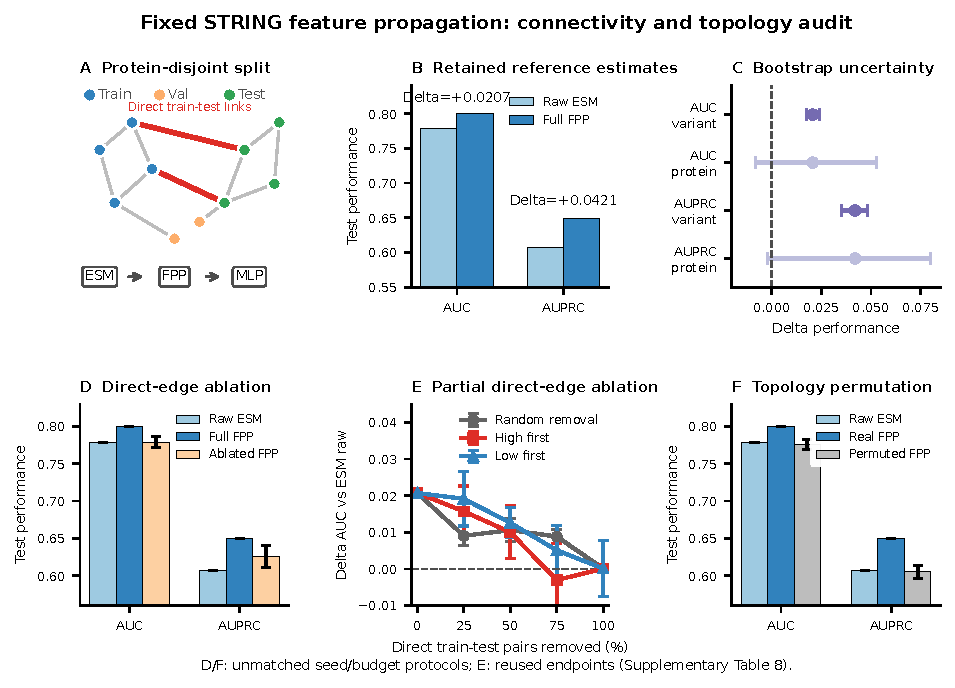
\includegraphics[width=0.98\textwidth]{figure_drafts/Figure1_fixed_propagation_audit.pdf}
\caption{Workflow and primary audit of fixed STRING feature propagation. A, Audit design: ClinVar variants are mapped to STRING proteins, ESM protein representations are propagated over a shared STRING graph, downstream MLP classifiers are trained on variant labels, and graph-specific effects are tested by connectivity ablation, protein-clustered uncertainty analysis and topology permutation. B, Retained reference run in which full-graph FPP improves over raw ESM; repeated classifier seeds show the same direction with a smaller mean AUC difference, as reported in the text and Supplementary Table 2. C, Variant-level bootstrap supports positive gain, whereas protein-clustered bootstrap widens uncertainty across zero. D, Direct-edge ablation: five runs, max 30 epochs, compared with single reference estimates. E, Intermediate ablation fractions: three runs per strategy/fraction; endpoints reuse existing estimates. F, Permutation: three graphs by three classifier runs, max 30 epochs. D--F are descriptive comparisons with unequal seed/budget protocols (Supplementary Table 8).}
\label{fig:connectivity}
\end{figure*}

\subsection{Architecture-matched fusion and homology-aware stress test}

Under the original split, the external variant-effect predictors provided strong baselines. The single-score CADD and AlphaMissense baselines achieved CADD-only AUC 0.9207 and AUPRC 0.8049, and AlphaMissense-only AUC 0.9470 and AUPRC 0.8899. In the matched repeated-run fusion-control audit used for Fig. 2, an architecture-matched \CADDAM{} baseline trained with the same 512/128 MLP used for fusion controls achieved mean AUC 0.9572 and AUPRC 0.9068. Adding raw ESM representation to \CADDAM{} improved performance to AUC 0.9680 and AUPRC 0.9317, showing complementarity between protein-level sequence representation and the two scalar predictors. Real FPP fusion achieved AUC 0.9718 and AUPRC 0.9415; edge-ablated graph fusion reached AUC 0.9708 and AUPRC 0.9395, and topology-permuted graph fusion reached AUC 0.9694 and AUPRC 0.9355. Paired bootstrap using ensemble-averaged predictions gave a real-fusion margin over raw ESM fusion (protein-clustered $\Delta$ AUC 95\% CI 0.0005 to 0.0075; $\Delta$ AUPRC CI 0.0032 to 0.0167). The smaller margins over edge-ablated and topology-permuted graph controls crossed zero under protein-clustered uncertainty. Protein-representation controls retained substantial fusion gains. The real-network margins over ablated and permuted controls are unresolved, rather than demonstrated absent or equivalent (Fig. 2B,C).

Under the homology-aware split, FPP remained higher than raw ESM, increasing AUC from 0.7248 to 0.7606 and AUPRC from 0.2418 to 0.2768 (Fig. 2D). With CADD and AlphaMissense included, the retained graph-fusion estimate was lower than the repeated-run architecture-matched two-predictor baseline. The architecture-matched \CADDAM{} baseline achieved AUC 0.9754 and AUPRC 0.8401; \CADDAM{} plus raw ESM achieved mean AUC 0.9728 and AUPRC 0.8249; and the retained graph-fusion model achieved AUC 0.9741 and AUPRC 0.8333 (Fig. 2E). These are within-split descriptive contrasts: one graph-fusion run cannot establish a stable ordering against repeated baseline means. The prevalence shift restricts cross-split AUPRC interpretation but does not invalidate comparisons on the same test set.

\begin{figure*}[!t]
\centering
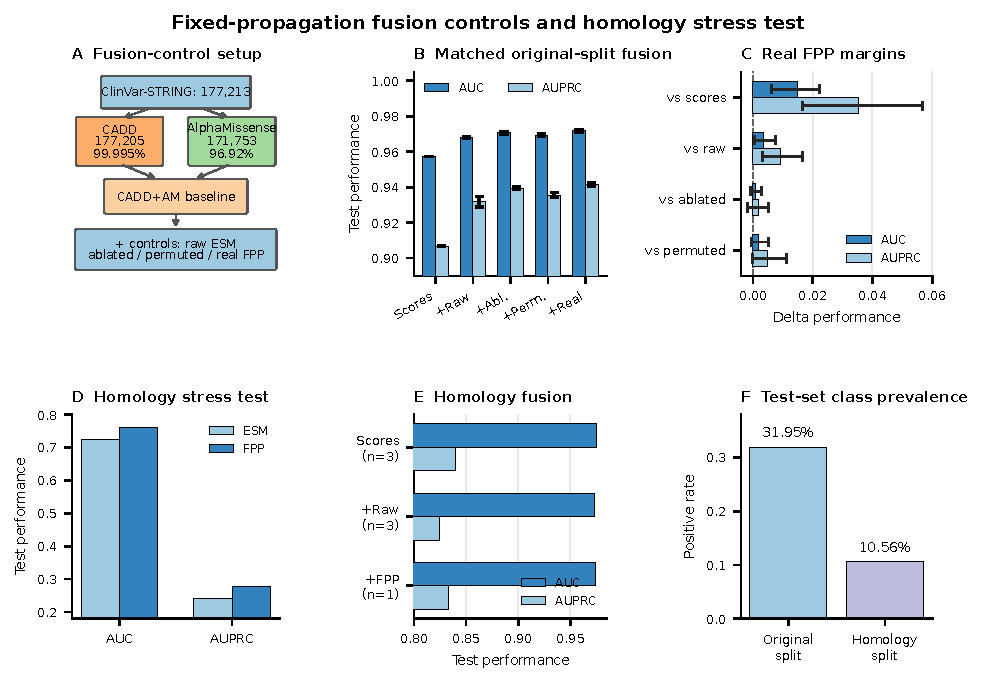
\includegraphics[width=0.98\textwidth]{figure_drafts/Figure2_fusion_homology.pdf}
\caption{Fixed-propagation fusion controls and descriptive homology-aware evaluation. A, CADD and AlphaMissense matching and fusion-control setup. B, Original-split repeated-run performance of architecture-matched \CADDAM{}, \CADDAM{}+raw ESM, \CADDAM{}+edge-ablated FPP, \CADDAM{}+topology-permuted FPP and \CADDAM{}+real FPP. Bars show mean test performance across three matched classifier seeds except topology-permuted fusion, which uses three topology permutations by three classifier seeds (n=9); error bars indicate one standard deviation. C, Marginal test-set gain of real FPP fusion over architecture-matched \CADDAM{} and protein-representation controls; error bars show protein-clustered paired-bootstrap 95\% confidence intervals computed from ensemble-averaged test predictions. Because panel C computes metrics from ensemble-averaged probabilities, its point deltas need not equal differences between the across-seed mean metrics shown in panel B. Intervals condition on fitted prediction ensembles and the sampled graph permutations; they do not include retraining or new-permutation uncertainty and do not test equivalence. D, Homology-aware split comparison of raw ESM and FPP. E, Homology-aware architecture-matched \CADDAM{}, \CADDAM{}+raw ESM and graph fusion; \CADDAM{} and \CADDAM{}+raw ESM are repeated-run means, whereas graph fusion is the retained homology-aware point estimate. F, Test-set prevalence differs by split. Scores denotes CADD+AlphaMissense; Raw, Abl., Perm. and Real denote the representations added to those scores.}
\label{fig:fusion_homology}
\end{figure*}

\subsection{Exploratory topology-context descriptions}

ESM representation space showed weak but detectable correspondence with STRING topology. Sampled STRING-neighbour pairs had mean ESM cosine similarity 0.8789 compared with 0.8639 for random protein pairs, and within-community pairs had higher similarity than between-community pairs (0.8743 versus 0.8642; Fig. 3A). This pattern is consistent with modest correspondence between ESM representation space and STRING network structure before propagation.

Graph-derived gains were not monotonic with simple centrality. Mid-k-core variants showed $\Delta$ AUC +0.0775 and $\Delta$ AUPRC +0.1049, whereas high-degree variants showed $\Delta$ AUC -0.0178 (Fig. 3B). Betweenness and clustering also shaped gain profiles: low- and mid-betweenness groups showed positive AUC gains (+0.0614 and +0.0522), while high betweenness showed a negative AUC difference (-0.0145); mid- and high-clustering groups showed positive gains, while low clustering was close to zero (Fig. 3C).

Neighbour-risk stratification and joint topology maps localized the graph signal to specific contexts. Low-, mid- and high-neighbour-risk strata all had positive AUC gains (+0.0641, +0.0265 and +0.0284), with different AUC and AUPRC profiles across strata (Fig. 3D). Exploratory joint topology maps identified stronger positive and negative profiles, including mid-k-core plus high-betweenness variants ($\Delta$ AUC +0.1429), mid-k-core plus mid-clustering variants (+0.1408), high-neighbour-risk plus mid-k-core variants (+0.1274), and high-k-core plus low-clustering variants (-0.0532; Fig. 3E,F). These 53 evaluated joint cells and highlighted profiles were inspected on the same test data. Their intervals quantify within-cell resampling only; neither those intervals nor feature-level FDR correction accounts for selection of high-gain cells. Independent subgroup confirmation is required.

\begin{figure*}[!t]
\centering
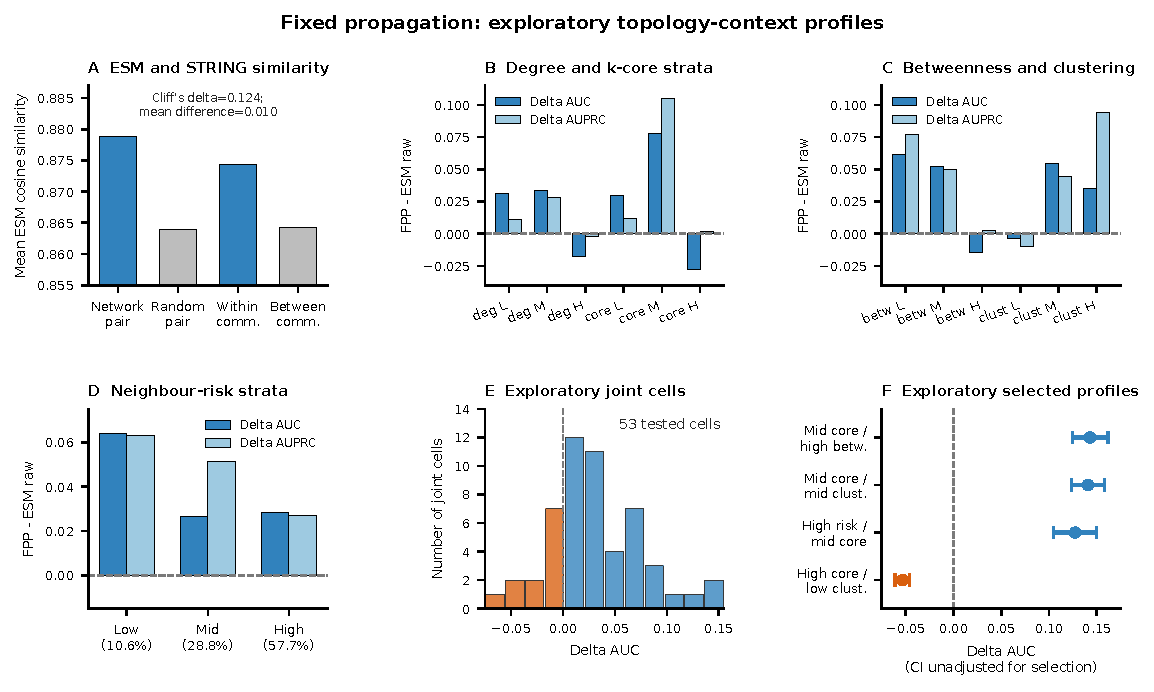
\includegraphics[width=0.98\textwidth]{figure_drafts/Figure3_exploratory_topology.pdf}
\caption{Exploratory descriptions of FPP gains across network topology contexts. A, ESM representations show weak alignment with STRING topology. B, Degree and k-core gains are non-monotonic. C, Betweenness and clustering strata shape graph-derived gain. D, Neighbour-risk strata show local-context dependence. E, Exploratory joint-cell distribution. L/M/H denote low/mid/high strata; deg, core, betw and clust denote degree, k-core, betweenness and clustering. F, Exploratory selected profiles; intervals are unadjusted for test-set selection and require independent validation.}
\label{fig:topology_context}
\end{figure*}

\subsection{Graph augmentation reshapes false-negative and false-positive predictions differently}

At a fixed decision-score threshold of 0.5, raw ESM and FPP were jointly correct for 11,875 test variants and jointly wrong for 3,965 variants. FPP corrected 1,436 variants and degraded 944 variants relative to raw ESM. Corrected variants included 837 pathogenic false negatives rescued and 599 benign false positives suppressed, whereas degraded variants included 904 benign true negatives converted to false positives and 40 pathogenic true positives converted to false negatives (Fig. 4A).

The retained-reference \CADDAM{} baseline and graph-fusion model were jointly correct for 15,981 variants and jointly wrong for 1,298 variants; graph fusion corrected 666 variants and degraded 275 variants. The corrected set contained more suppressed false positives than rescued false negatives (444 versus 222; Fig. 4B). Figure 4B uses this retained-reference model pair, while Figure 2 reports the architecture-matched repeated-run comparison.

Topology profiles differed between rescued false negatives and suppressed false positives. In the raw ESM to FPP comparison, rescued false negatives had higher degree, neighbour-risk, neighbour pathogenic rate, neighbour training-variant count and betweenness; suppressed false positives had higher clustering coefficient and within-community neighbour fraction (Fig. 4C). Similar profile shifts appeared in the retained \CADDAM{} to graph-fusion comparison (Fig. 4D). Multiple topology features remained significant after FDR correction (Fig. 4E), and baseline-error-stratified contrasts showed differences across degree, k-core, neighbour-risk, neighbour pathogenic rate, betweenness and boundary role (Fig. 4F). These are descriptive associations within baseline false-negative or false-positive groups, without continuous-score matching. A post-hoc threshold sweep from 0.1 to 0.9 (Supplementary Table 10) found net corrections of -234 at 0.1 and +10 to +587 at 0.2--0.9 for raw ESM to FPP. The retained fusion pair had positive net corrections throughout, but its dominant corrected error type reversed at 0.7. Thus the detailed error-type story at 0.5 is threshold-dependent.

\begin{figure*}[!t]
\centering
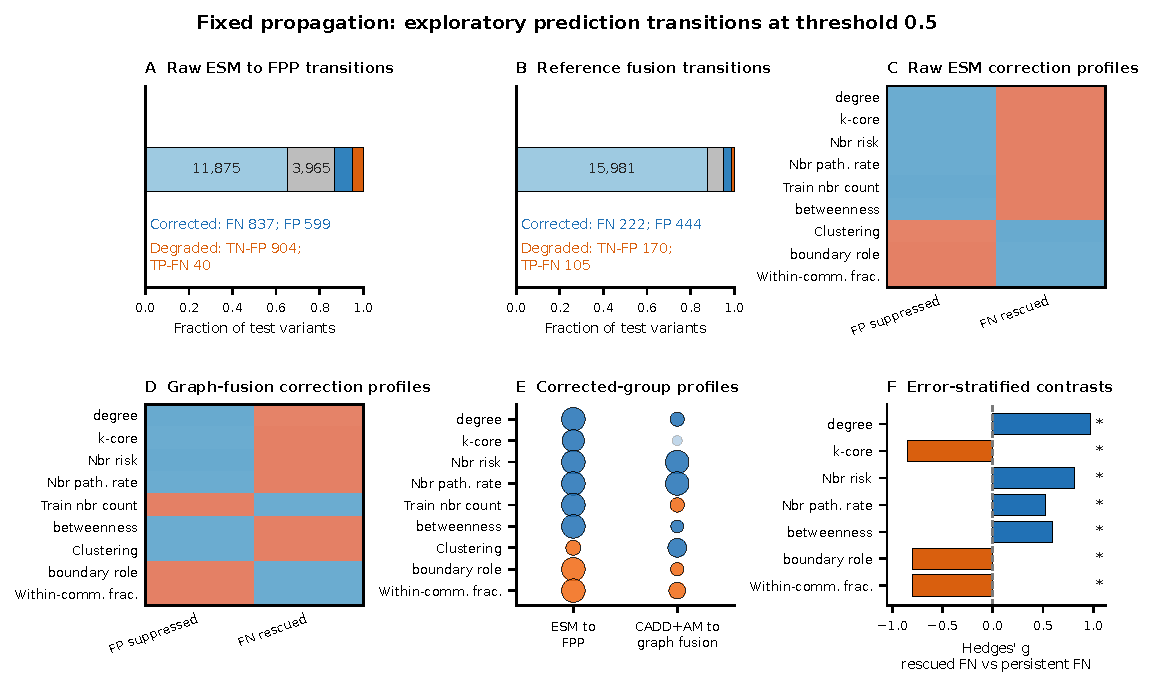
\includegraphics[width=0.98\textwidth]{figure_drafts/Figure4_prediction_transitions.pdf}
\caption{Graph augmentation changes false-negative and false-positive predictions in different network contexts. A, Prediction transitions from raw ESM to FPP at a fixed decision-score threshold of 0.5. B, Transitions for the retained-reference \CADDAM{} and graph-fusion model pair. C-D, Row-normalized heatmaps compare topology profiles of suppressed false positives and rescued false negatives. E, Corrected groups differ across multiple topology features after FDR correction. F, Baseline-error-stratified contrasts, without continuous-score matching. Nbr denotes neighbour; path. rate is training-neighbour pathogenic rate. Counts are threshold-specific and sigmoid outputs are uncalibrated; see Supplementary Table 10.}
\label{fig:prediction_transitions}
\end{figure*}

\section{Discussion}

This audit concerns fixed feature propagation on one STRING association network. The original-split repeated comparison improved over raw ESM, whereas connectivity and identity-permutation controls produced lower performance under different training protocols. These findings motivate matched graph controls; they do not identify a purely causal connectivity effect. Shared graph structure and held-out protein features are permitted by the transductive design. No test labels enter propagation, but deployment to newly arriving, disconnected proteins is not evaluated.

Architecture-matched fusion shows complementarity between protein representations and external scores. In a post-hoc complete-case test subset of 17,581 variants, without retraining, mean AUC/AUPRC were 0.9597/0.9118 for \CADDAM{}, 0.9694/0.9344 for raw-ESM fusion, 0.9720/0.9420 for edge-ablated fusion, 0.9708/0.9382 for permuted fusion and 0.9730/0.9438 for real FPP fusion (Supplementary Table 9). The point ordering is preserved, but this restricted evaluation does not test an alternative complete-case training procedure. Intervals crossing zero for small real-network margins establish uncertainty, not equivalence or a performance ceiling.

The external predictors are not independent prospective references. CADD uses proxy-neutral versus simulated proxy-deleterious training examples and incorporates ESM-1v features \cite{Kircher2014CADD,Schubach2024CADDv17}; AlphaMissense uses population-derived weak supervision and clinical variants for model selection and calibration \cite{Cheng2023AlphaMissense}. Clinical-data involvement in development differs from direct supervised training on our labels. Historical clinical overlap was not enumerated or excluded here. A temporal cohort excluding predictor-development variants is needed before interpreting these comparisons as prospective generalization.

The homology-aware split changes protein composition and prevalence, and its graph fusion has only one retained run. It supplies descriptive within-split evidence, not a reproducible inferiority claim or a cross-split AUPRC ranking. Matched repeated runs and prevalence-controlled comparisons remain necessary. The topology profiles and error transitions are exploratory; independent data must test subgroup reproducibility, and threshold-dependent transitions must not be treated as calibrated clinical improvements.

Several further boundaries matter. STRING combines functional associations beyond physical interactions; physical-only and alternative networks were not tested \cite{Szklarczyk2023STRING}. Fixed propagation may be inadequate to extract useful topology even when that topology is informative. The supplementary mean and cosine-weighted operators are also fixed: they are not trained GraphSAGE or GAT baselines. Learned attention, heterogeneous variant graphs and context-aware models therefore remain outside the scope of the present conclusions. Protein-level features omit mutation identity and isoform effects, while ClinVar submission bias, changing labels and the review-status whitelist limit transfer \cite{Landrum2020ClinVar}. Binary labels discard graded functional effects; stricter/looser training filters and independent functional assays were not evaluated. Computational pathogenicity predictions require clinical or functional confirmation and cannot alone establish diagnosis or treatment.

\section*{Data and Code Availability}

A compact anonymized source-data archive containing figure source data, summary metrics, bootstrap outputs and checksums has been prepared. The archive includes revised figure generators and reproducible post-hoc sensitivity inputs. Large-scale reconstruction and training require the original provider resources and an appropriate compute environment. Large third-party resources, including CADD, AlphaMissense, ClinVar and STRING source files, should be obtained from their original providers.

\section*{AI-Tool Disclosure}

OpenAI ChatGPT, OpenAI Codex and Anthropic Claude supported literature organization, analysis-code drafting and language editing. Original model experiments were performed by the authors. Revision-stage sensitivity statistics were recomputed from frozen outputs using AI-assisted local scripts with row-alignment and metric-reproduction checks. The authors retain responsibility for study design, interpretation, citation verification and final approval. The tools are not authors; no new model training or synthetic outcomes were introduced in this revision.

\begin{thebibliography}{99}
\bibitem{Barabasi2011NetworkMedicine} A.-L. Barabasi, N. Gulbahce, and J. Loscalzo, ``Network medicine: a network-based approach to human disease,'' \emph{Nature Reviews Genetics}, vol. 12, pp. 56--68, 2011, doi: 10.1038/nrg2918.
\bibitem{Benjamini1995FDR} Y. Benjamini and Y. Hochberg, ``Controlling the false discovery rate: a practical and powerful approach to multiple testing,'' \emph{Journal of the Royal Statistical Society: Series B}, vol. 57, pp. 289--300, 1995, doi: 10.1111/j.2517-6161.1995.tb02031.x.
\bibitem{Chen2018InteractomePerturbation} S. Chen et al., ``An interactome perturbation framework prioritizes damaging missense mutations for developmental disorders,'' \emph{Nature Genetics}, vol. 50, pp. 1032--1040, 2018, doi: 10.1038/s41588-018-0130-z.
\bibitem{Cheng2021VEGN} J. Cheng, C. Lawrence, and M. Niepert, ``VEGN: variant effect prediction with graph neural networks,'' arXiv:2106.13642, 2021, doi: 10.48550/arXiv.2106.13642.
\bibitem{Cheng2023AlphaMissense} J. Cheng et al., ``Accurate proteome-wide missense variant effect prediction with AlphaMissense,'' \emph{Science}, vol. 381, eadg7492, 2023, doi: 10.1126/science.adg7492.
\bibitem{Efron1993Bootstrap} B. Efron and R. J. Tibshirani, \emph{An Introduction to the Bootstrap}. Chapman \& Hall/CRC, 1993.
\bibitem{Frazer2021EVE} J. Frazer et al., ``Disease variant prediction with deep generative models of evolutionary data,'' \emph{Nature}, vol. 599, pp. 91--95, 2021, doi: 10.1038/s41586-021-04043-8.
\bibitem{Ghadie2025DiseaseSpecificGNN} M. Ghadie, S. Sardaar, and Y. Trakadis, ``Disease-specific prediction of missense variant pathogenicity with DNA language models and graph neural networks,'' \emph{Bioengineering}, vol. 12, p. 1098, 2025, doi: 10.3390/bioengineering12101098.
\bibitem{Ioannidis2016REVEL} N. M. Ioannidis et al., ``REVEL: an ensemble method for predicting the pathogenicity of rare missense variants,'' \emph{American Journal of Human Genetics}, vol. 99, pp. 877--885, 2016, doi: 10.1016/j.ajhg.2016.08.016.
\bibitem{Kingma2015Adam} D. P. Kingma and J. Ba, ``Adam: a method for stochastic optimization,'' \emph{International Conference on Learning Representations}, 2015, arXiv:1412.6980.
\bibitem{Kipf2017GCN} T. N. Kipf and M. Welling, ``Semi-supervised classification with graph convolutional networks,'' \emph{International Conference on Learning Representations}, 2017.
\bibitem{Kircher2014CADD} M. Kircher et al., ``A general framework for estimating the relative pathogenicity of human genetic variants,'' \emph{Nature Genetics}, vol. 46, pp. 310--315, 2014, doi: 10.1038/ng.2892.
\bibitem{Landrum2020ClinVar} M. J. Landrum et al., ``ClinVar: improvements to accessing data,'' \emph{Nucleic Acids Research}, vol. 48, pp. D835--D844, 2020, doi: 10.1093/nar/gkz972.
\bibitem{Lin2023ESM} Z. Lin et al., ``Evolutionary-scale prediction of atomic-level protein structure with a language model,'' \emph{Science}, vol. 379, pp. 1123--1130, 2023, doi: 10.1126/science.ade2574.
\bibitem{Littmann2022ProteinMLTips} Q. Hou, K. Waury, D. Gogishvili, and K. A. Feenstra, ``Ten quick tips for sequence-based prediction of protein properties using machine learning,'' \emph{PLOS Computational Biology}, vol. 18, no. 12, Art. no. e1010669, 2022, doi: 10.1371/journal.pcbi.1010669.
\bibitem{Menche2015DiseaseModules} J. Menche et al., ``Disease networks. Uncovering disease-disease relationships through the incomplete interactome,'' \emph{Science}, vol. 347, 1257601, 2015, doi: 10.1126/science.1257601.
\bibitem{Ozturk2022NetworkFeatures} K. Ozturk and H. Carter, ``Predicting functional consequences of mutations using molecular interaction network features,'' \emph{Human Genetics}, vol. 141, pp. 1195--1210, 2022, doi: 10.1007/s00439-021-02329-5.
\bibitem{Qi2021MVP} H. Qi et al., ``MVP predicts the pathogenicity of missense variants by deep learning,'' \emph{Nature Communications}, vol. 12, p. 510, 2021, doi: 10.1038/s41467-020-20847-0.
\bibitem{Sahni2015InteractionPerturbation} N. Sahni et al., ``Widespread macromolecular interaction perturbations in human genetic disorders,'' \emph{Cell}, vol. 161, pp. 647--660, 2015, doi: 10.1016/j.cell.2015.04.013.
\bibitem{Saito2015PrecisionRecall} T. Saito and M. Rehmsmeier, ``The precision-recall plot is more informative than the ROC plot when evaluating binary classifiers on imbalanced datasets,'' \emph{PLOS ONE}, vol. 10, e0118432, 2015, doi: 10.1371/journal.pone.0118432.
\bibitem{Schubach2024CADDv17} M. Schubach et al., ``CADD v1.7: using protein language models, regulatory CNNs and other nucleotide-level scores to improve genome-wide variant predictions,'' \emph{Nucleic Acids Research}, vol. 52, no. D1, pp. D1143--D1154, 2024, doi: 10.1093/nar/gkad989.
\bibitem{Steinegger2017MMseqs2} M. Steinegger and J. Soding, ``MMseqs2 enables sensitive protein sequence searching for the analysis of massive data sets,'' \emph{Nature Biotechnology}, vol. 35, pp. 1026--1028, 2017, doi: 10.1038/nbt.3988.
\bibitem{Sundaram2018PrimateAI} L. Sundaram et al., ``Predicting the clinical impact of human mutation with deep neural networks,'' \emph{Nature Genetics}, vol. 50, pp. 1161--1170, 2018, doi: 10.1038/s41588-018-0167-z.
\bibitem{Szklarczyk2023STRING} D. Szklarczyk et al., ``The STRING database in 2023: protein-protein association networks and functional enrichment analyses for any sequenced genome of interest,'' \emph{Nucleic Acids Research}, vol. 51, pp. D638--D646, 2023, doi: 10.1093/nar/gkac1000.
\bibitem{Teufel2023GraphPart} F. Teufel, M. H. Gislason, J. J. Almagro Armenteros, A. R. Johansen, O. Winther, and H. Nielsen, ``GraphPart: homology partitioning for biological sequence analysis,'' \emph{NAR Genomics and Bioinformatics}, vol. 5, lqad088, 2023, doi: 10.1093/nargab/lqad088.
\bibitem{Yates2014SuSPect} C. M. Yates, I. Filippis, L. A. Kelley, and M. J. E. Sternberg, ``SuSPect: enhanced prediction of single amino acid variant phenotype using network features,'' \emph{Journal of Molecular Biology}, vol. 426, pp. 2692--2701, 2014, doi: 10.1016/j.jmb.2014.04.026.
\bibitem{Yu2025GNNMAP} H. Yu et al., ``A graph neural network approach for accurate prediction of pathogenicity in multi-type variants,'' \emph{Briefings in Bioinformatics}, vol. 26, bbaf151, 2025, doi: 10.1093/bib/bbaf151.
\bibitem{Zhang2022gMVP} H. Zhang, M. S. Xu, X. Fan, W. K. Chung, and Y. Shen, ``Predicting functional effect of missense variants using graph attention neural networks,'' \emph{Nature Machine Intelligence}, vol. 4, no. 11, pp. 1017--1028, 2022, doi: 10.1038/s42256-022-00561-w.
\end{thebibliography}
\end{document}
